\chapter{Protección de sobreintensidadesde líneas de AT}
\section{Protección contra sobreintensidades}
Los dispositivos de protección deberán eliminar las sobreintensidades sin que se produzcan PROYECCIONES PELIGROSAS NI EXPLOSIONES. Se establecerá una adecuada coordinación entre las protecciones para que la parte desconectada en caso de cortocircuito o sobrecarga sea la menor posible y tener selectividad.
\newline

Protecciones a las salidas de líneas:
\begin{itemize}
	\item Se protegerán contra cortocircuitos y, cuando proceda, contra sobrecargas
	\item Redes de 1ª (66-220kV) y 2ª Categoría (30-66kV): esta protección se hará con Interruptores Automáticos
	\item Líneas aéreas de transporte o de distribución pública: protección contra defectos transitorios equipados con dispositivos de reenganche automático (podrá omitirse o bloquearse cuando esté justificado técnicamente).
	\item Redes de distribución pública de 3ª Categoría (1-30kV): se establecerá una normalización de las potencias máximas de cortocircuito en barras de salida, para las diversas tensiones
	\item Protección de líneas en redes con neutro a tierra:
	\begin{itemize}
		\item Protección contra cortocircuitos a tierra que puedan producirse en cualquiera de las fases
		\item El funcionamiento de la protección no debe aislar el neutro de tierra
	\end{itemize}
	\item Protección de líneas en redes con neutro aislado:
	\begin{itemize}
		\item En el caso de utilizar interruptores automáticos para la protección contra cortocircuitos a tierra, será suficiente relés sobre dos de las fases
		\item En el caso de líneas aéreas sistema detector de tensión homopolar en la subestación donde esté la cabeza de línea. Si la subestación es sin vigilancia la protección debe provocar apertura de interruptores automáticos.
	\end{itemize}
\end{itemize}
\section{Protección de sobreintensidad de tiempo inverso}
\begin{itemize}
	\item El tiempo de respuesta depende del valor de la intensidad:
	Mayor intensidad menor tiempo de respuesta
	\item Protección de sobrecargas
	\begin{itemize}
		\item Faltas a tierra en redes con neutro impedante
		\item Faltas de alta impedancia en redes con neutro rígido
		\item Subtensiones
		\item Funcionamiento en monofásico
		\item Cargas superiores a las previstas
	\end{itemize}
\end{itemize}
\subsection{Curvas características}
\begin{figure}[H]
	\centering
	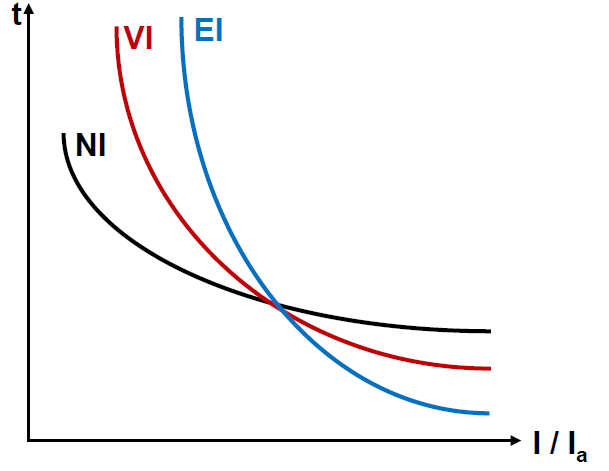
\includegraphics[width=0.7\linewidth]{Images/61}
	\label{fig:61}
\end{figure}
\begin{equation}
	t_a=\dfrac{k}{\left(\dfrac{I}{I_{ar}}\right)^n-1}\cdot t_{ik}
\end{equation}

Donde $t_a$ es el tiempo de actuación, $k$ y $n$ factores de forma, $I$ la intensidad que circula por el relé, $I_{ar}$ la intensidad de arranque programada en el relé y $t_{ik}$ un factor de tiempo.
\newline

Tipos de curvas
\begin{itemize}
	\item Normalmente Inversa – NI ($k = 0,14\, , n = 0,02$): Sobreintensidades cercanas a la generación del sistema
	\item Muy Inversa – VI ($k = 13,50\, , n = 1,00$): Faltas relativamente alejadas de la generación del sistema
	\item Extremadamente Inversa – EI ($k = 80,00\, , n = 2,00$): Faltas alejadas de generación, permiten reenganchar cargas sin disparos en la fase de conexión y selectividad con fusibles. Alimentadores de distribución.
\end{itemize}

Aplicaciones:
\begin{itemize}
	\item Protección principal de líneas de 3ª categoría
	\item Protección de apoyo en líneas y barras de 1ª y 2ª categoría
	\item Protección de faltas impedantes en generadores, motores, transformadores y cables
\end{itemize}

Tiempo despeje falta:
\begin{equation}
	t_t=t_a+t_{dInterruptor}
\end{equation}
\newpage
\section{Protección de sobreintensidad de tiempo fijo}
\begin{figure}[H]
	\centering
	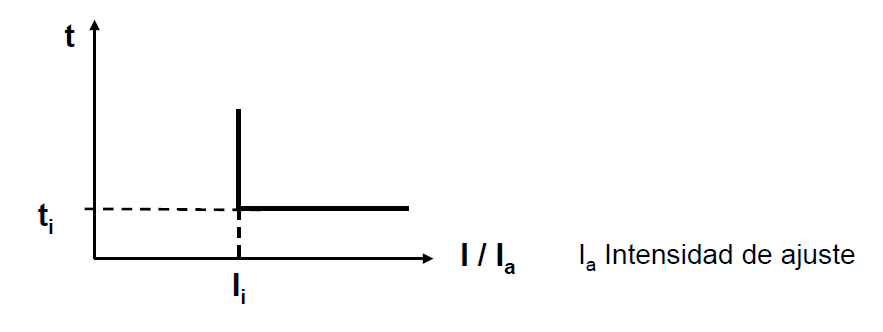
\includegraphics[width=0.7\linewidth]{Images/62}
	\label{fig:62}
\end{figure}
\begin{itemize}
	\item Protección frente a cortocircuitos
	\item El tiempo de respuesta independiente del valor de la intensidad
	\item Ajustes de intensidad y tiempo (selectividad)
	\item Normalmente se usa selectividad cronométrica
\end{itemize}
\subsection{Relés de sobreintensidad de neutro 50N/51N}
\begin{itemize}
	\item Se emplea en redes de distribución con alta intensidad de defecto a tierra: redes con neutro rígido o de baja impedancia
	\item Disparo imperativo: este relé actúa sobre el interruptor automático
	\item Vigila la intensidad de fallo a tierra. Mide la intensidad homopolar
	\item Situación del transformador de intensidad:
	\begin{itemize}
		\item TI con núcleo toroidal sobre el neutro
		\item TI suma sobre las fases
	\end{itemize}
	\item Ajustes: permite ajustar la intensidad y el tiempo de retardo
	\item Selectividad: se consigue aumentando el tiempo de respuesta
	\item No es un relé direccional
\end{itemize}
\section{Protección de sobreintensidad direccional}
Como se alimenta desde los dos extremos para no dejar ramas sin alimentar es necesario tener relés direccionales para cortar donde sea necesario. Se mejora la selectividad.
\begin{figure}[H]
	\centering
	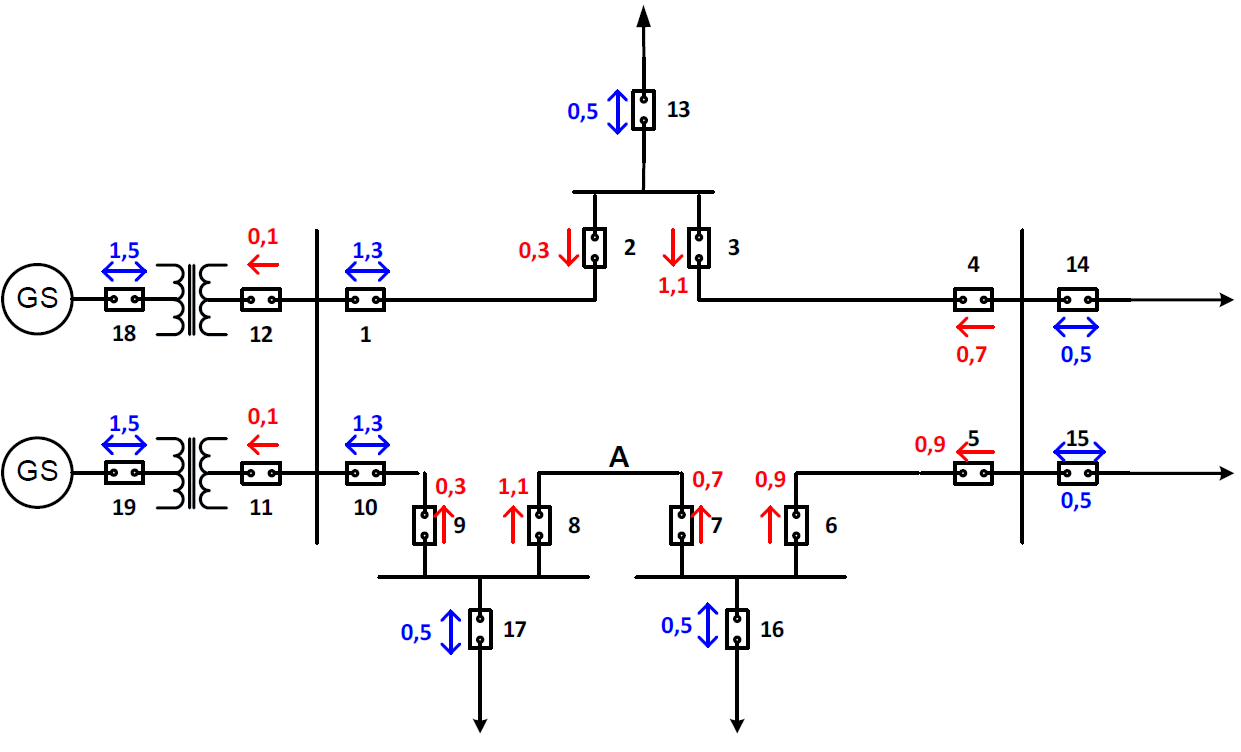
\includegraphics[width=0.7\linewidth]{Images/63}
	\label{fig:63}
\end{figure}

\begin{figure}[H]
	\centering
	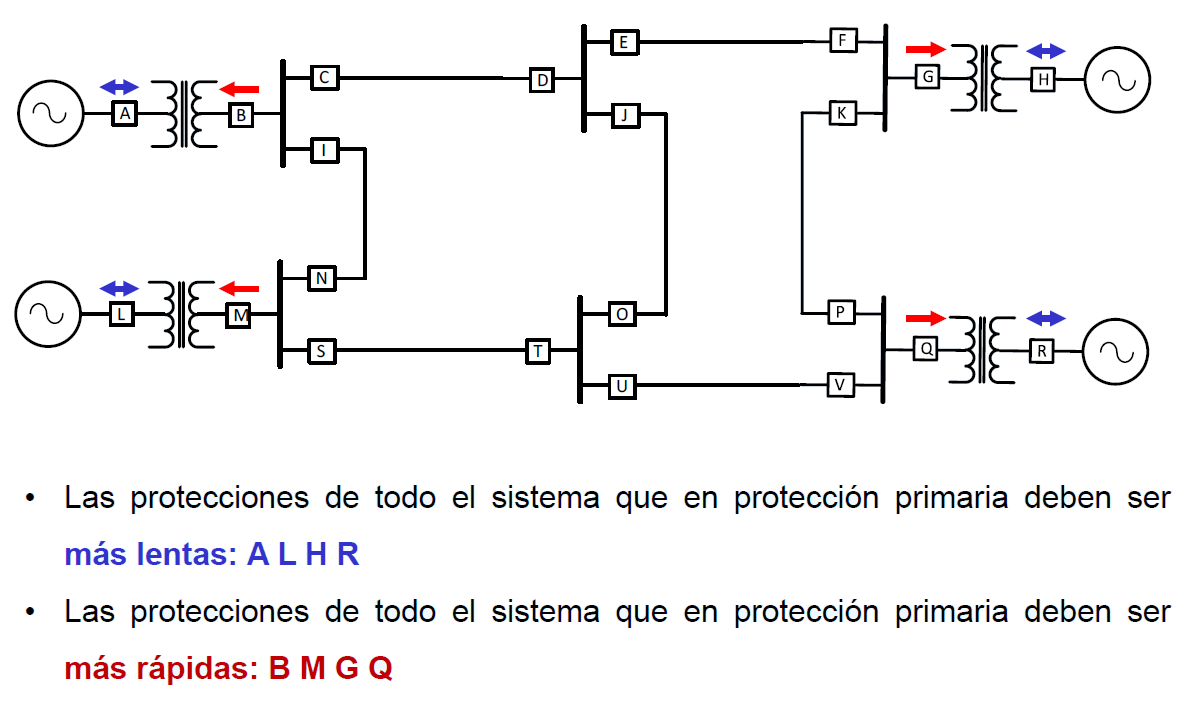
\includegraphics[width=0.7\linewidth]{Images/64}
	\label{fig:64}
\end{figure}

Los relés solo actúan cuando la intensidad de falta circula en una dirección determinada:
\begin{itemize}
	\item Requieren monitorización de intensidad y de tensión
	\item Incluyen control de sobreintensidad y control direccional
	\item Si se alimentan de la red: tensión del orden del 0,25 \% para funcionar adecuadamente
	\item En el caso anterior miden tensiones compuestas
	\item Se emplea con altas intensidades de defecto (neutro rígido a tierra o impedante) en redes de distribución en paralelo
	\item Mide la intensidad homopolar y las tensiones de línea:
	\begin{itemize}
		\item Tensión de línea por TT
		\item Intensidad homopolar por TI toroidal o suma
	\end{itemize}
	\item Ajuste del ángulo de disparo
\end{itemize}
\begin{figure}[H]
	\centering
	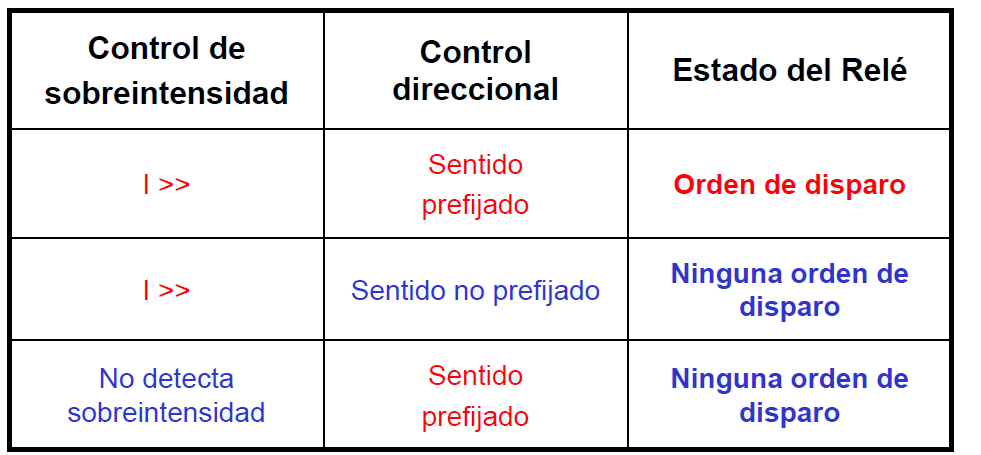
\includegraphics[width=0.5\linewidth]{Images/66}
	\label{fig:66}
\end{figure}

\begin{figure}[H]
	\centering
	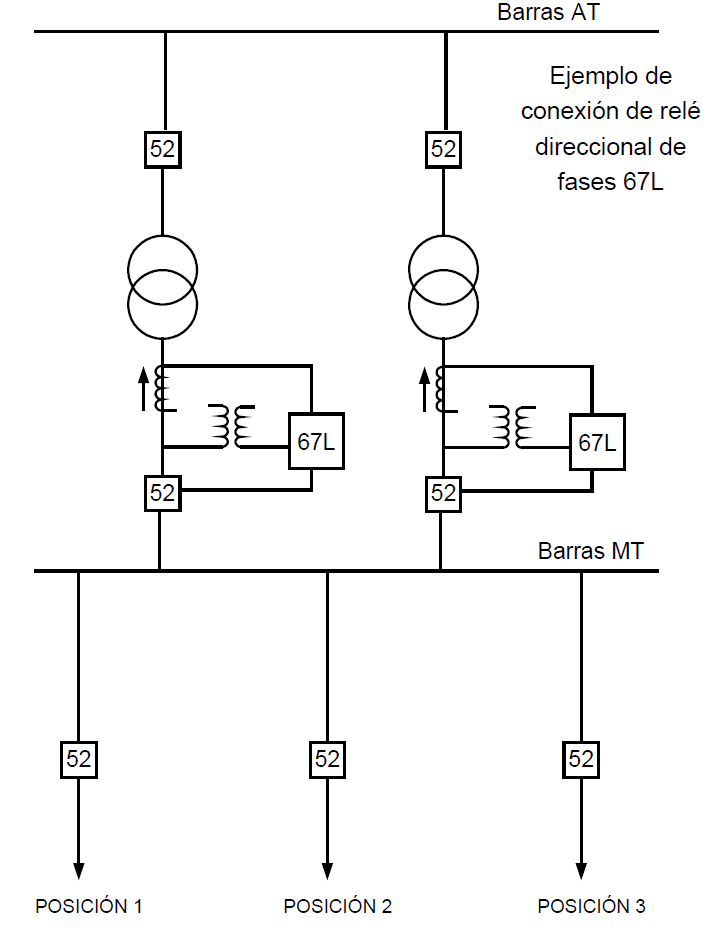
\includegraphics[width=0.3\linewidth]{Images/65}
	\label{fig:65}
\end{figure}
